%!TEX options = -shell-escape

\documentclass[12pt]{report}
\usepackage[a4paper,twoside,top=20mm,bottom=20mm,inner=30mm,outer=25mm]{geometry}
\usepackage[utf8]{inputenc}
\usepackage[greek,english]{babel}
\usepackage[scaled=0.86]{couriers}
\usepackage[toc,page,title,titletoc]{appendix}
\usepackage[pdfpagelabels,unicode]{hyperref}
\usepackage{bookmark}
\usepackage[fixlanguage]{babelbib}
\selectbiblanguage{greek}
\usepackage{titlesec}
\usepackage{etoolbox}
\usepackage{graphicx}
\usepackage{array}
\usepackage{amsmath}
\usepackage{minted}
\usepackage{subcaption}
\captionsetup{compatibility=false}
\graphicspath{ {images/} }
\usepackage[noend]{algpseudocode}
\usepackage{algorithm}
\usepackage{afterpage}
\usepackage{comment}

\newcommand\blankpage{%
    \null
    \thispagestyle{empty}%
    \addtocounter{page}{-1}%
    \newpage}

\hypersetup{
  colorlinks=true,
  % linkcolor=green,
  citecolor=red,
  % filecolor=blue,
  urlcolor=blue,
  % pdftitle=,
  % pdfauthor=,
  % pdfsubject=,
  % pdfkeywords=
}

\setcounter{secnumdepth}{3}
\setcounter{tocdepth}{3}

\titleformat{\chapter}
  {\normalfont\LARGE\bfseries}{\thechapter}{1em}{}
\titlespacing*{\chapter}{0pt}{3.5ex plus 1ex minus .2ex}{2.3ex plus .2ex}

\makeatletter
\patchcmd\@resets@pp{%
  \def\Hy@chapapp{\appendixname }%
}{%
  \def\Hy@chapapp{appendix}%
}{}{\errmessage{Cannot patch \string\@resets@pp}}
\patchcmd\@resets@ppsub{%
  \def\Hy@chapapp{\appendixname }%
}{%
  \def\Hy@chapapp{appendix}%
}{}{\errmessage{Cannot patch \string\@resets@pp}}
\makeatother

\addto{\captionsgreek}{\renewcommand{\appendixpagename}{Παραρτήματα}}
\addto{\captionsgreek}{\renewcommand{\appendixtocname}{Παραρτήματα}}
\addto{\captionsgreek}{\renewcommand{\appendixname}{Παράρτημα}}

\begin{document}
\selectlanguage{greek}

\hypersetup{pageanchor=false}

\begin{titlepage}
  \centering
  
\includegraphics[width=0.15\textwidth]{pyrforos}\par\vspace{1cm}
  {\scshape\LARGE Εθνικό Μετσόβιο Πολυτεχνείο\\
  Σχολή Ηλεκτρολόγων Μηχανικών και Μηχανικών Η/Υ\par}
  \vspace{1cm}
  {\scshape\Large Εργασία στο Μεταπτυχιακό Μάθημα\\
  Διαχείριση Τεχνολογιών στο Ηλεκτρονικό Εμπόριο\par}
  \vspace{1.5cm}
  {\Large\bfseries Ανάπτυξη Ιστοσελίδας Ηλεκτρονικών Δημοπρασιών\par}
  \vspace{2cm}
  {\large Δημήτριος Πολίτης (ΥΔ)\par}
  \vfill
  Επιβλέπων \par
  Καθ. Ευστάθιος Συκάς

  \vfill

% Bottom of the page
  {\large \today\par}
  \afterpage{\blankpage}
\end{titlepage}

\tableofcontents
\thispagestyle{empty}

\listoftables
\thispagestyle{empty}

\listoffigures
\thispagestyle{empty}

\begin{abstract}
Στο παρόν παρουσιάζεται η λειτουργία και η διαδικασία ανάπτυξης μιας ιστοσελίδας δημοπρασιών. Αρχικά  γίνεται αναφορά στις βασικές έννοιες του ηλεκτρονικού εμπορίου Παρουσιάζονται αρχικά τα διαθέσιμα λογισμικά, τα πλεονεκτήματα και μειονεκτήματά τους και στη συνέχεια περιγράφεται αναλυτικά η διαδικασία δημιουργίας ενός ιστοτόπου ηλεκτρονικών δημοπρασιών με τη χρήση αυτοματοποιημένων εργαλείων (\textlatin{phpProBid, vagrant}).

\vspace{10mm}

\noindent \textbf{Λέξεις κλειδιά:} Ηλεκτρονικό Εμπόριο, Ηλεκτρονική Δημοπρασία, Ανοιχτός Κώδικας, Εξυπηρετητής Ιστοσελίδων, Διαδίκτυο.
\end{abstract}

\hypersetup{pageanchor=true}
\clearpage
\pagenumbering{arabic}

\chapter{Εισαγωγή}\label{ch1}
\section{Εισαγωγή}
Η εποχή του διαδικτύου επιβάλει την αναθεώρηση των παραδοσιακών τρόπων διεξαγωγής του εμπορίου, μέσω φυσικής επαφής. Πλέον μεγάλο ποσοστό των εμπορικών συναλλαγών, τόσο μεταξύ επιχειρήσεων, όσο και μεταξύ ιδιωτών και επιχειρήσεων, πραγματοποιούνται με ηλεκτρονικά μέσα.

Η δημιουργία, η συντήρηση και η ανανέωση του περιεχομένου των ιστοτόπων ηλεκτρονικών αγορών αποτελεί μοχλό μεγέθυνσης των πωλήσεων και σε βάθος χρόνου, του κύκλου εργασιών.

\section{Ηλεκτρονικό Εμπόριο}
\subsection{Ορισμοί - Έννοιες}
Το Ηλεκτρονικό Εμπόριο (ΗΕ) περιγράφει τη διαδικασία αγοράς, πώλησης, μεταφοράς ή ανταλλαγής προϊόντων , υπηρεσιών ή/και πληροφοριών μέσω δικτύων υπολογιστών, περιλαμβανομένου και του Διαδικτύου~\cite{turban_outland_king_lee_liang_turban_2018}. Το ΗΕ μπορεί να οριστεί από τις παρακάτω σκοπιές:
  \paragraph{Επιχειρησιακή Διεργασία.} Από την σκοπιά των επιχειρησιακών διεργασιών το ΗΕ αφορά στην εκτέλεση των διεργασιών με ηλεκτρονικό τρόπο, ολοκληρώνοντας ηλεκτρονικές διεργασίες μέσω δικτύων Η/Υ.
  \paragraph{Εξυπηρέτηση.} Από τη σκοπιά των επιχειρήσεων, το ΗΕ είναι ένα εργαλείο που απευθύνεται στη επιθυμία των κυβερνήσεων, των εταιριών, των πελατών και της διοίκησης να περικόψουν το κόστος των υπηρεσιών ενώ ταυτόχρονα να βελτιώσουν την παρεχόμενη ποιότητα των υπηρεσιών και ταχύτητα εξυπηρέτησης.
  \paragraph{Εκπαίδευση.} Από τη σκοπιά της εκπαίδευσης, το ΗΕ παρέχει την δυνατότητα εκπαίδευσης και επιμόρφωσης \textlatin{online} σε σχολεία, πανεπιστήμια και επιχειρήσεις.
  \paragraph{Συνεργατική.} Από τη σκοπιά της συνεργασίας είναι το πλαίσιο της ενδοεπιχειρησιακής και διαεπιχειρησιακής συνέχειας.
  \paragraph{Κοινωνική.} Από την κοινωνική σκοπιά, το ΗΕ παρέχει μια θέση συγκέντρωσης μελών της κοινωνίας για εκμάθηση, συνδιαλλαγή και συνεργασία.

Πολλές φορές το ΗΕ συγχέεται με το Ηλεκτρονικό Επιχειρείν, μια πιο ευρεία έννοια. Το Ηλεκτρονικό Επιχειρείν αναφέρεται στον ευρύτερο ορισμό του ΗΕ, όχι μόνο στην αγορά και την πώληση των αγαθών αλλά και επίσης στην εξυπηρέτηση πελατών, στη συνεργασία με επιχειρηματικούς εταίρους, στη διεξαγωγή ηλεκτρονικής εκπαίδευσης και την διεξαγωγή ηλεκτρονικών συναλλαγών εντός των ορίων του οργανισμού.

Σύμφωνα με το~\cite{chen_2005} το Ηλεκτρονικό Επιχειρείν είναι η χρήση του Διαδικτύου και άλλων τεχνολογιών της πληροφορικής για την υποστήριξη του εμπορίου και τη βελτίωση της απόδοσης μιας επιχείρησης.

\subsection{Αμιγές και Μερικό ΗΕ}
Το ηλεκτρονικό εμπόριο μπορεί να πάρει πολλές μορφές ανάλογα με το βαθμό ψηφιοποίησης των παρακάτω παραγόντων:
\begin{itemize}
  \item του προϊόντος - υπηρεσίας προς πώληση
  \item της διαδικασίας (για παράδειγμα παραγγελία ή πληρωμή)
  \item της μεθόδου διανομής
\end{itemize}

Στο~\cite{choi_stahl_whinston_1997} παρουσιάζεται ένα μοντέλο που περιγράφει τους πιθανούς συνδυασμούς αυτών των τριών διαστάσεων. Ένα προϊόν μπορεί να είναι φυσικό ή ψηφιακό, η μέθοδος διανομής μπορεί να είναι φυσική η ηλεκτρονική, Η διαδικασία μπορεί αναλόγως να είναι φυσική η ψηφιακή. Αυτές οι εναλλακτικές καταστασεις δημιουργούν οκτώ τρισδιάστατους κύβους. Στο παραδοσιακό εμπόριο όλες οι διαστάσεις είναι φυσικές, ενώ στο αμιγές ΗΕ όλες οι διαστάσεις είναι ψηφιακές. Όλοι οι άλλοι κύβοι περιλαμβάνουν ένα μείγμα ψηφιακών και φυσικών διαστάσεων. Η περιγραφή αυτή γίνεται κατανοητή εφόσον παρατηρήσουμε το σχήμα~\ref{fig:ec_dimensions}.
\begin{figure}[h]
\centering
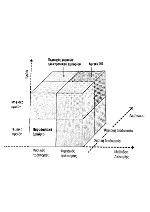
\includegraphics[width=0.8\textwidth, height=8cm]{ec-dimensions}
\caption{Διάγραμμα τύπων ΗΕ}
\label{fig:ec_dimensions}
\end{figure}
Εάν υπάρχει έστω και μια ψηφιακή διάσταση, τότε έχουμε μερικό ΗΕ. Αναλόγως με τον τρόπο τον οποίο διεξάγουν την πώληση και τη διανομή ενός εμπορεύματος, οι οργανισμοί - εταιρίες μπορούν να να κατηγοριοποιηθούν όπως παρακάτω:
\begin{itemize}
  \item Παραδοσιακοί Οργανισμοί (παλαιάς οικονομίας).
  \item Εικονικοί ή ηλεκτρονικοί οργανισμοί.
  \item Οργανισμοί μερικού ΗΕ.
\end{itemize}
Οι αμιγώς φυσικοί οργανισμοί αναφέρονται ως παραδοσιακοί οργανισμοί, ενώ εταιρίες οι οποίες χρησιμοποιούν μόνο ΗΕ θεωρούνται εικονικοί οργανισμοί. Οι οργανισμοί μερικού ΗΕ είναι εκείνοι οι οργανισμοί που επιτελούν μερικές δραστηριότητες ηλεκτρονικού εμπορίου, ενώ οι κύρια δραστηριότητά τους πραγματοποιείται με φυσικό τρόπο.

\subsection{Τύποι Ηλεκτρονικού Εμπορίου}
Μια συνηθισμένη κατάταξη του ΗΕ είναι με βάση την φύση της συνναλλαγής ή με τη σχέση ανάμεσα στους συμμετέχοντες, όπως παρακάτω:
\begin{itemize}
  \item \textlatin{Bussiness to Bussiness (B2B)}, Όλοι οι συμμετέχοντες είναι επιχειρήσεις ή άλλοι οργανισμοί.
  \item \textlatin{Bussiness to Consumer (B2C)}, Περιλαμβάνει συναλλαγές λιανικού εμπορίου προϊόντων ή υπηρεσιών από επιχειρήσεις προς μεμονομένους αγοραστές.
  \item \textlatin{Bussiness to Government (B2G)}, Περιλαμβάνει συναλλαγές παροχής υπηρεσιών ή αγαθών από επιχειρήσεις προς το δημόσιο τομέα.
  \item \textlatin{Government to Bussiness (G2B)}, Περιλαμβάνει συναλλαγές παροχής υπηρεσιών από το κράτος προς τον ιδιωτικό τομέα.
  \item \textlatin{Consumer to Consumer (C2C)}, Περιλαμβάνει συναλλαγές λιανικού εμπορίου προϊόντων ή υπηρεσιών από ιδιώτες προς ιδιώτες.
  \item \textlatin{Government to Consumer (G2C)}, Περιλαμβάνει συναλλαγές παροχής υπηρεσιών από το κράτος προς τον ιδιώτες.
\end{itemize}

\section{Ηλεκτρονικές Θέσεις Αγορών}
Σύμφωνα με τον~\cite{bakos_1998}, οι αγορές διαδραματίζουν ουσιώδη ρόλο στην οικονομία διευκολύνοντας την ανταλλαγή πληροφοριών, αγαθών, υπηρεσιών και πληρωμών. Οι αγορές (ηλεκτρονικές ή όχι) έχουν τρεις κύριες λειτουργίες:
\begin{itemize}
  \item Ταίριασμα αγοραστών - πωλητών.
  \item Παροχή ενός θεσμικού πλαισίου (νομικού - ρυθμιστικού) για την αποτελεσματική λειτουργία τους.
  \item Διευκόλυνση ανταλλαγή πληροφοριών, αγαθών κτλ, όπως αναφέρθηκε παραπάνω.
\end{itemize}

\subsection{Ηλεκτρονικές Θέσεις Αγορών}
Η βασική θέση για τη διεξαγωγή συναλλαγών ΗΕ είναι η ηλεκτρονική αγορά. Μια Ηλεκτρονική θέση Αγορών είναι μια εικονική θέση αγορών, στην οποία συναντώνται και διεξάγουν διάφορους τύπους συναλλαγών πωλητές και αγοραστές. Η λειτουργίες μιας ηλεκτρονικής θέσης αγορών είναι πανομοιότυπες με αυτές μιας φυσικής αγοράς. Τα ηλεκτρονικά μέσα όμως κάνουν τις αγορές περισσότερο αποδοτικές, παρέχοντας πλήθος ενημερωμένων πληροφοριών σε όλους τους εμπλεκομένους. Διακρίνονται σε:
\begin{itemize}
  \item Ιδιωτικές: Η θέση αγορών ανήκει σε ένα μόνο φορέα - εταιρία, η οποία τη διαχειρίζεται και είτε πωλεί τα δικά της προϊόντα (ένας προς πολλούς), είτε προσκαλεί προμηθευτές (πολλοί προς έναν).
  \item Δημόσιες: Ανήκουν σε κάποιο τρίτο και περιλαμβάνουν πολλούς αγοραστές και πωλητές.
  \item Θέσεις αγορών με πράκτορες: Οι πράκτορες λογισμικού συγκεντρώνουν πληροφορίες σχετικά με προϊόντα και τιμές και να τα παρουσιάζουν σε πιθανούς αγοραστές ή πωλητές. Στην πιο εξελιγμένη τους μορφή οι πράκτορες αγοραστή και πωλητή μπορούν να αλληλεπιδρούν σε μια πλήρως αυτοματοποιημένη αγορά~\cite{turban_outland_king_lee_liang_turban_2018}.
\end{itemize}

\subsection{Οι Δημοπρασίες ως Μηχανισμοί Αγορών ΗΕ}
Ένας από τους πιο ενδιαφέροντες μηχανισμούς της αγοράς στο ηλεκτρονικό εμπόριο είναι οι ηλεκτρονικές δημοπρασίες. Αυτές Χρησιμοποιούνται στα \textlatin{B2C, B2B, C2C, G2B, G2C} κ.α. Μια δημοπρασία είναι ένας μηχανισμός αγοράς, που χρησιμοποιεί μια ανταγωνιστική διαδικασία κατά την οποία, ένας πωλητής δέχεται ακολουθιακές προσφορές από αγοραστές (προωθητική δημοπρασία) ή ένας αγοραστής δέχεται προσφορές από πωλητές (αντίστροφη δημοπρασία). Είναι δυνατό να λάβουν χώρα:
\begin{itemize}
  \item Σε δημόσιες τοποθεσίες δημοπρασιών, όπως το \textlatin{EBay}.
  \item Κατόπιν προσκλήσης σε ιδιωτικές δημοπρασίες.
\end{itemize}

Το παρόν πραγματεύεται την ανάπτυξη μιας ιστοσελίδας ηλεκτρονικών δημοπρασιών πλήρους λειτουργικότητας. Στα επόμενα παρουσιάζεται η διαδικασία ανάπτυξης, τα εργαλεία που χρησιμοποιήθηκαν και γίνεται μια συνοπτική αναφορά στις λειτουργίες που παρέχει η υπόψη ιστοσελίδα ηλεκτρονικών δημοπρασιών.

\chapter{Ανάπτυξη Ιστοσελίδας Ηλεκτρονικών Δημοπρασιών}\label{ch2}
Για την ανάπτυξη της ιστοσελίδας της εργασίας χρησιμοποιήθηκε πλήθος εργαλείων, τα οποία στην πλειονότητά τους βρίσκονται διαθέσιμα δωρεάν στο Διαδίκτυο (\textlatin{Open Source Software}). Στα επόμενα γίνεται μια σύντομη αναφορά στα εργαλεία ανάπτυξης που χρησιμοποιήθηκαν.

\section{\textlatin{\textlatin{Vagrant (Open Source VM Provissioner}}}
Το \textlatin{Vagrant} είναι ένα εργαλείο δημιουργίας και διαχείρησης εικονικών μηχανών με τη χρήση μιας εξαιρετικά απλοποιημένης διαδικασίας~\cite{vagrant_by_hashicorp}. Το εργαλείο αυτό δίνει έμφαση στην αυτοματοποιημένη διαχείριση των εικονικών μηχανών και μειώνει σημαντικά το χρόνο δημιουργίας και παραμετροποίησης ενός \textlatin{development server}.

Είναι γραμμένο στη γλώσσα προγραμματισμού \textlatin{Ruby} και αποτελεί έναν ενιαίο τρόπο επικοινωνίας με δίάφορους \textlatin{providers} εικονικών μηχανών (όπως \textlatin{VirtualBox, VMware, AWS} κ.α.). Με τον τρόπο αυτό είναι δυνατή η δημιουργία εικονικών μηχανών με τις επιθυμητές παραμέτρους στον μικρότερο δυνατό χρόνο. Παράλληλα, για την εγκατάσταση πακέτων λογισμικού αλλά και παραμετροποίηση σε επίπεδο λειτουργικού συστήματος (ΛΣ), είναι δυνατή η συνεργασία με ευρέως διαδεδομένα \textlatin{provisioning tools}, όπως \textlatin{Chef, Puppet, Ansible} ακόμα και με απλά \textlatin{shell scripts}.

Το μεγαλύτερο ίσως πλεονέκτημα του υπόψη εργαλείου είναι η δυνατότητα παροχής στους προγραμματιστές ενός ενιαίου περιβάλλοντος, το οποίο είναι σταθερό και όσο κοντά γίνεται στο παραγωγικό εξυπηρετητή. Επίσης επειδή η παραμετροποίηση γίνεται με αυτόματο τρόπο, αφαιρείται από τους προγραμματιστές το βάρος της δημιουργίας, συντήρησης και αποσφαλμάτωσης του περιβάλλοντος ανάπτυξης.

Η αρχή λειτουργίας του \textlatin{Vagrant} στηρίζεται στην ύπαρξη μιας εικονικής μηχανής στελέχους (\textlatin{template / vagrant box}), η οποία είναι διαθέσιμη από τα επίσημα αποθετήρια~\url{\textlatin{https://atlas.hashicorp.com}} είτε μπορεί να είναι δική μας. Κατόπιν μέσω μιας διαδικασίας κλωνοποίησης και εφαρμογής παραμέτρων, εντελώς διαφανούς για το χρήστη, αποδίδεται η εικονική μηχανή στο χρήστη.

Όλα τα παραπάνω γίνονται με την εκελεση της εντολής \
Για τη φιλοξενία του ιστοτόπου της εργασ

\section{Συμπεράσματα}
Στο παρόν, παρουσιάστηκε ένα μοντέλο προσομοίωσης του πρωτοκόλλου πολλαπλής πρόσβασης μέσου (\textlatin{MAC}) τύπου \textlatin{slotted aloha}. Τα αποτελέσματα της προσομοίωσης έδειξαν τιμές πολύ κοντά στις θεωρητικά αναμενόμενες. Συγκεκριμένα, η αύξηση των μνημών προσωρινής αποθήκευσης πακέτων (\textlatin{receiving buffers}) στους σταθμούς, είχε θετική επίδραση στην απόδοση του συστήματος \textlatin{S}, η οποία όμως εμφανίζονταν φθίνουσα, καθώς αυξάνονταν το πλήθος των σταθμών \textlatin{M}. Επίσης, η αύξηση του πλήθους των \textlatin{receiving buffers} πάνω από δύο, δεν είχε κάποια σημαντική επίδραση στην αποδοτικότητα του συστήματος. Αντιθέτως, η αύξηση των διαύλων επικοινωνίας μεταξύ των κόμβων είχε σημαντικά θετική επίδραση στην διεκπεραιωτική δυνατότητα του συστήματος και τη μείωση της καθυστέρησης, ανεξάρτητα από το πλήθος των σταθμών.

Τα παραπάνω καταδεικνύουν ότι η βέλτιστη απόδοση του πρωτοκόλλου επιτυγχάνεται όταν οι σταθμοί έχουν δύο το πλήθος \textlatin{receiving buffers} και ικανό αριθμό καναλιών - διαύλων επικοινωνίας μεταξύ τους (ο οποίος μπορεί να περιορίζεται από τεχνικούς περιορισμούς ή περιορισμούς κόστους). Στην περίπτωση των ασύρματων δικτύων αυτό μπορεί να μεταφραστεί: είτε σε ικανό αριθμό πομποδεκτών ανά σταθμό, οι οποίοι θα λειτουργούν σε διαφορετικές συχνότητες για λόγους αποφυγής παρεμβολών, είτε σε κατάλληλο σχήμα πολύπλεξης (\textlatin{TDM, FDM}), επαναχρησιμοποίηση φάσματος με αναπήδηση συχνότητας κ.α. Κατά αντιστοιχία, στα οπτικά δίκτυα είναι δυνατή η χρησιμοποίηση πολύτροπων οπτικών ινών και εκπομπή των δεδομένων σε διαφορετικά μήκη κύματος για την ταυτόχρονη χρησιμοποίηση του μέσου.

\begin{appendices}

\end{appendices}

\appendix

\bibliographystyle{babplain}
\bibliography{e-commerce}

\end{document}